\documentclass[aspectratio=169, 12pt]{beamer}

% ---------- theme + colours ----------
\usetheme{Madrid}
\definecolor{tenderlyForest}{HTML}{205C4D}
\definecolor{tenderlyCream}{HTML}{FBF7EF}
\definecolor{tenderlyTerra}{HTML}{B8533E}
\definecolor{tenderlyInk}{HTML}{18332A}

\setbeamercolor{palette primary}{bg=tenderlyForest, fg=white}
\setbeamercolor{palette secondary}{bg=tenderlyForest!80, fg=white}
\setbeamercolor{palette tertiary}{bg=tenderlyForest!60, fg=white}
\setbeamercolor{structure}{fg=tenderlyForest}
\setbeamercolor{title}{fg=tenderlyInk}
\setbeamercolor{frametitle}{bg=tenderlyForest, fg=white}
\setbeamercolor{block title}{bg=tenderlyForest, fg=white}
\setbeamercolor{block body}{bg=tenderlyCream}
\setbeamercolor{alerted text}{fg=tenderlyTerra}
\setbeamercolor{item}{fg=tenderlyForest}
\setbeamercolor{background canvas}{bg=white}

\setbeamerfont{title}{series=\bfseries, size=\Large}
\setbeamerfont{frametitle}{series=\bfseries}

% ---------- packages ----------
\usepackage[utf8]{inputenc}
\usepackage[T1]{fontenc}
\usepackage{graphicx}
\usepackage{tikz}
\usetikzlibrary{arrows.meta, positioning, shapes.geometric, calc, fit}
\usepackage{booktabs}
\usepackage{amsmath}

% ---------- metadata ----------
\title{Tenderly}
\subtitle{AI-Powered Volunteer Matching for San Francisco}
\author{Team Tenderly}
\date{AI for Social Good --- MLH \& DigitalOcean Hackathon 2026}

% ================================================================
\begin{document}

% ---------- title slide ----------
\begin{frame}[plain]
  \begin{center}
    \vspace{1.5cm}
    {\Huge\bfseries\color{tenderlyInk} Tenderly}\\[0.4cm]
    {\large\color{tenderlyForest} AI-Powered Volunteer Matching for San Francisco}\\[1.2cm]
    {\normalsize\color{tenderlyTerra}\textbf{When someone has the willingness to help,\\Tenderly turns uncertainty into a clear next step.}}\\[1.5cm]
    {\small AI for Social Good --- MLH \& DigitalOcean Hackathon $\cdot$ July 2026}
  \end{center}
\end{frame}

% ---------- the problem ----------
\begin{frame}{The Problem}
  \begin{columns}[T]
    \begin{column}{0.55\textwidth}
      \textbf{People want to help but hit three kinds of friction:}
      \begin{enumerate}
        \item They don't know which organization needs \emph{their} particular skills
        \item Long, undifferentiated opportunity lists feel overwhelming
        \item Urgency is invisible --- volunteers can't tell when a small commitment could matter most
      \end{enumerate}
      \vspace{0.4cm}
      Meanwhile, nonprofits must explain needs repeatedly and compete for attention even as conditions change across the city.
    \end{column}
    \begin{column}{0.4\textwidth}
      \begin{block}{The Gap}
        \centering
        \textbf{50 listings to browse}\\
        $\downarrow$\\[0.2cm]
        \alert{No clear next step}\\[0.2cm]
        $\downarrow$\\
        \textbf{Volunteer gives up}
      \end{block}
    \end{column}
  \end{columns}
\end{frame}

% ---------- user journey ----------
\begin{frame}{User Journey}
  \begin{center}
  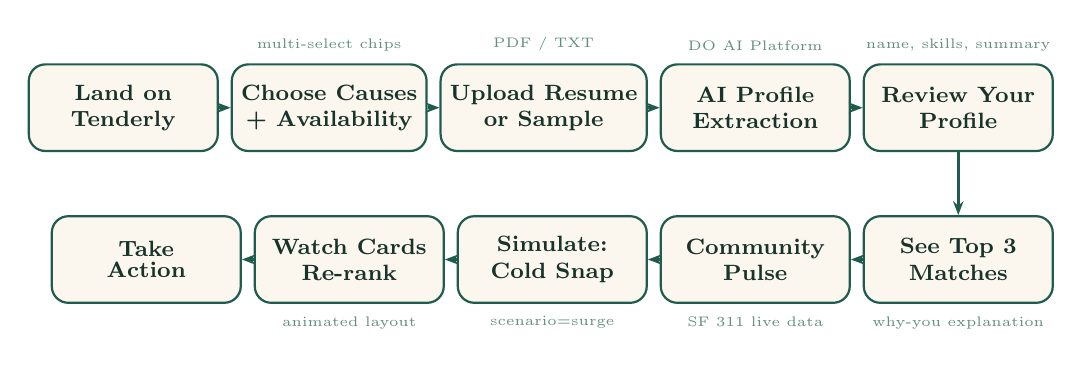
\begin{tikzpicture}[
    node distance=0.3cm and 0.15cm,
    flowstep/.style={
      rounded corners=6pt,
      draw=tenderlyForest,
      fill=tenderlyCream,
      text=tenderlyInk,
      minimum height=1.1cm,
      minimum width=2.4cm,
      align=center,
      font=\footnotesize\bfseries,
      line width=0.8pt,
    },
    arr/.style={
      -{Stealth[length=5pt]},
      tenderlyForest,
      line width=1pt,
    },
    lbl/.style={
      font=\tiny,
      text=tenderlyForest!70,
      align=center,
    },
  ]
    % row 1
    \node[flowstep] (land) {Land on\\Tenderly};
    \node[flowstep, right=of land] (causes) {Choose Causes\\+ Availability};
    \node[flowstep, right=of causes] (upload) {Upload Resume\\or Sample};
    \node[flowstep, right=of upload] (loading) {AI Profile\\Extraction};
    \node[flowstep, right=of loading] (profile) {Review Your\\Profile};

    % row 2
    \node[flowstep, below=0.8cm of profile] (matches) {See Top 3\\Matches};
    \node[flowstep, left=of matches] (pulse) {Community\\Pulse};
    \node[flowstep, left=of pulse] (surge) {Simulate:\\Cold Snap};
    \node[flowstep, left=of surge] (rerank) {Watch Cards\\Re-rank};
    \node[flowstep, left=of rerank] (act) {\alert{Take}\\[-2pt]\alert{Action}};

    % arrows row 1
    \draw[arr] (land) -- (causes);
    \draw[arr] (causes) -- (upload);
    \draw[arr] (upload) -- (loading);
    \draw[arr] (loading) -- (profile);

    % connector
    \draw[arr] (profile) -- (matches);

    % arrows row 2
    \draw[arr] (matches) -- (pulse);
    \draw[arr] (pulse) -- (surge);
    \draw[arr] (surge) -- (rerank);
    \draw[arr] (rerank) -- (act);

    % labels
    \node[lbl, above=1pt of causes] {multi-select chips};
    \node[lbl, above=1pt of upload] {PDF / TXT};
    \node[lbl, above=1pt of loading] {DO AI Platform};
    \node[lbl, above=1pt of profile] {name, skills, summary};
    \node[lbl, below=1pt of matches] {why-you explanation};
    \node[lbl, below=1pt of pulse] {SF 311 live data};
    \node[lbl, below=1pt of surge] {scenario=surge};
    \node[lbl, below=1pt of rerank] {animated layout};
  \end{tikzpicture}
  \end{center}
\end{frame}

% ---------- DigitalOcean platform usage ----------
\begin{frame}{DigitalOcean Platform Usage}
  \begin{center}
  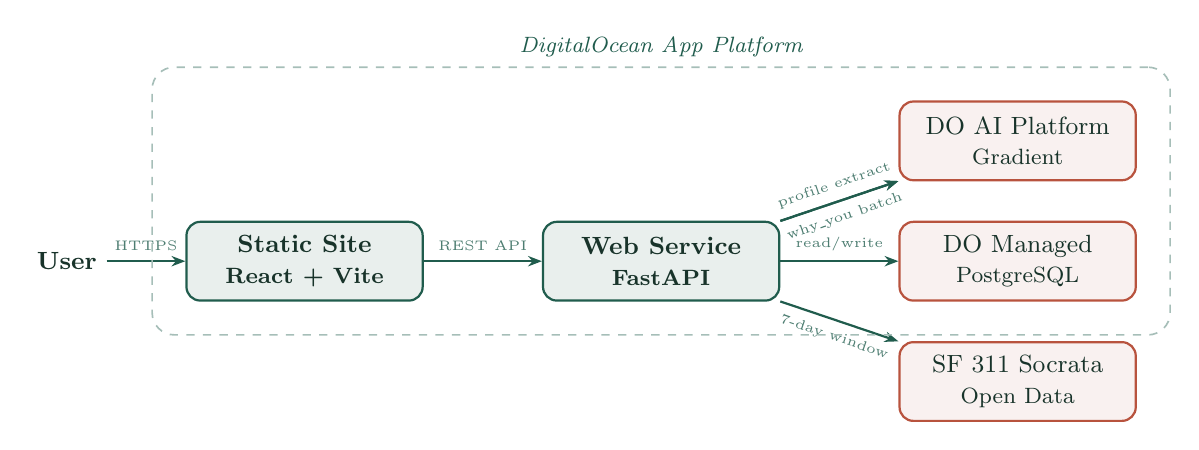
\begin{tikzpicture}[
    node distance=0.6cm and 0.8cm,
    svc/.style={
      rounded corners=5pt,
      draw=tenderlyForest,
      fill=tenderlyForest!10,
      text=tenderlyInk,
      minimum height=1cm,
      minimum width=3cm,
      align=center,
      font=\small\bfseries,
      line width=0.8pt,
    },
    ext/.style={svc, draw=tenderlyTerra, fill=tenderlyTerra!8, font=\small},
    arr/.style={-{Stealth[length=5pt]}, tenderlyForest, line width=0.8pt},
    lbl/.style={font=\tiny, text=tenderlyForest!80, midway},
  ]
    % frontend
    \node[svc] (fe) {Static Site\\{\footnotesize React + Vite}};

    % backend
    \node[svc, right=1.5cm of fe] (api) {Web Service\\{\footnotesize FastAPI}};

    % DO AI
    \node[ext, above right=0.5cm and 1.5cm of api] (ai) {DO AI Platform\\{\footnotesize Gradient}};

    % DO Postgres
    \node[ext, right=1.5cm of api] (db) {DO Managed\\{\footnotesize PostgreSQL}};

    % Socrata
    \node[ext, below right=0.5cm and 1.5cm of api] (soc) {SF 311 Socrata\\{\footnotesize Open Data}};

    % user
    \node[left=1cm of fe, font=\small\bfseries, text=tenderlyInk] (user) {User};

    % arrows
    \draw[arr] (user) -- node[lbl, above] {HTTPS} (fe);
    \draw[arr] (fe) -- node[lbl, above] {REST API} (api);
    \draw[arr] (api) -- node[lbl, above, sloped] {profile extract} (ai);
    \draw[arr] (api) -- node[lbl, below, sloped] {why\_you batch} (ai);
    \draw[arr] (api) -- node[lbl, above] {read/write} (db);
    \draw[arr] (api) -- node[lbl, below, sloped] {7-day window} (soc);

    % DO box
    \node[draw=tenderlyForest!40, dashed, rounded corners=8pt, line width=0.6pt,
          fit=(fe)(api)(ai)(db), inner sep=12pt, label={[font=\footnotesize\itshape, text=tenderlyForest]above:DigitalOcean App Platform}] {};
  \end{tikzpicture}
  \end{center}

  \vspace{0.2cm}
  \begin{columns}[T]
    \begin{column}{0.32\textwidth}
      \textbf{\color{tenderlyForest}Static Site}\\
      {\small Frontend built from Vite, serves \texttt{dist/}}
    \end{column}
    \begin{column}{0.32\textwidth}
      \textbf{\color{tenderlyForest}Web Service}\\
      {\small FastAPI backend on port 8080}
    \end{column}
    \begin{column}{0.32\textwidth}
      \textbf{\color{tenderlyForest}AI Platform}\\
      {\small 2 inference calls per user journey}
    \end{column}
  \end{columns}
\end{frame}

% ---------- AI: how matching works ----------
\begin{frame}{How Matching Works}
  \begin{columns}[T]
    \begin{column}{0.5\textwidth}
      \begin{block}{Weighted Match Score}
        \vspace{0.2cm}
        \[
          \text{score} = \underbrace{0.45}_{\text{skills}} + \underbrace{0.25}_{\text{causes}} + \underbrace{0.20}_{\text{availability}} + \underbrace{0.10}_{\text{location}}
        \]
        \vspace{0.1cm}
      \end{block}
      \vspace{0.3cm}
      \textbf{Skills} --- do your abilities match what the org needs?\\[0.2cm]
      \textbf{Causes} --- do you care about the same issues?\\[0.2cm]
      \textbf{Availability} --- can you show up when they need you?\\[0.2cm]
      \textbf{Location} --- how active is community need in that neighborhood?
    \end{column}
    \begin{column}{0.45\textwidth}
      \begin{block}{What Happens in a Cold Snap?}
        When conditions change in SF:
        \begin{itemize}
          \item Food and shelter roles get a \textbf{score boost}
          \item Neighborhoods with more reported need rise higher
          \item Urgency labels update (medium $\rightarrow$ high)
        \end{itemize}
      \end{block}
      \vspace{0.3cm}
      \begin{alertblock}{Explainable, Not a Black Box}
        Every recommendation comes with a plain-language reason: \emph{``Your project management skills and weekend availability make you a strong fit for this shelter coordination role.''}
      \end{alertblock}
    \end{column}
  \end{columns}
\end{frame}

% ---------- AI: 2 calls per journey ----------
\begin{frame}{DigitalOcean AI Platform --- Two Calls Per Journey}
  \begin{center}
  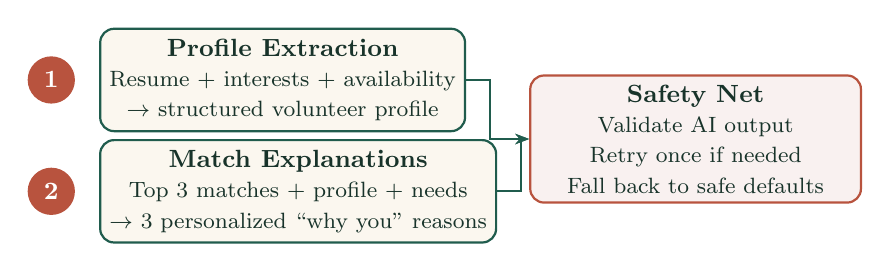
\begin{tikzpicture}[
    node distance=0.4cm and 0.6cm,
    box/.style={
      rounded corners=5pt,
      draw=tenderlyForest,
      fill=tenderlyCream,
      text=tenderlyInk,
      minimum height=1.3cm,
      minimum width=4.2cm,
      align=center,
      font=\small,
      line width=0.8pt,
    },
    arr/.style={-{Stealth[length=5pt]}, tenderlyForest, line width=0.8pt},
    num/.style={circle, fill=tenderlyTerra, text=white, font=\small\bfseries, inner sep=2pt, minimum size=0.6cm},
  ]
    % Call 1
    \node[num] (n1) {1};
    \node[box, right=0.3cm of n1] (c1) {\textbf{Profile Extraction}\\{\footnotesize Resume + interests + availability}\\{\footnotesize $\rightarrow$ structured volunteer profile}};

    % Call 2
    \node[num, below=0.8cm of n1] (n2) {2};
    \node[box, right=0.3cm of n2] (c2) {\textbf{Match Explanations}\\{\footnotesize Top 3 matches + profile + needs}\\{\footnotesize $\rightarrow$ 3 personalized ``why you'' reasons}};

    % Guardrails
    \node[box, right=0.8cm of c1, draw=tenderlyTerra, fill=tenderlyTerra!8, yshift=-0.75cm] (guard) {
      \textbf{Safety Net}\\
      {\footnotesize Validate AI output}\\
      {\footnotesize Retry once if needed}\\
      {\footnotesize Fall back to safe defaults}
    };

    \draw[arr] (c1.east) -- ++(0.3,0) |- (guard.west);
    \draw[arr] (c2.east) -- ++(0.3,0) |- (guard.west);
  \end{tikzpicture}
  \end{center}

  \vspace{0.3cm}
  \begin{center}
    \colorbox{tenderlyCream}{\parbox{0.85\textwidth}{\centering
    \small\textbf{Key guarantee:} If the AI service is down, every response falls back to pre-written defaults. The app keeps working --- the volunteer just sees a generic explanation instead of a personalized one.
    }}
  \end{center}
\end{frame}

% ---------- data ingestion pipeline ----------
\begin{frame}{How Opportunities Get Into Tenderly}
  \begin{columns}[T]
    \begin{column}{0.48\textwidth}
      \begin{center}
      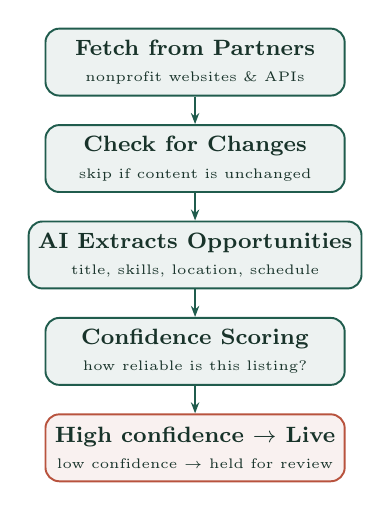
\begin{tikzpicture}[
        node distance=0.35cm,
        flowstep/.style={
          rounded corners=5pt,
          draw=tenderlyForest,
          fill=tenderlyForest!8,
          text=tenderlyInk,
          minimum height=0.85cm,
          minimum width=3.8cm,
          align=center,
          font=\footnotesize,
          line width=0.7pt,
        },
        db/.style={flowstep, draw=tenderlyTerra, fill=tenderlyTerra!8},
        arr/.style={-{Stealth[length=4pt]}, tenderlyForest, line width=0.7pt},
      ]
        \node[flowstep] (src) {\textbf{Fetch from Partners}\\{\tiny nonprofit websites \& APIs}};
        \node[flowstep, below=of src] (hash) {\textbf{Check for Changes}\\{\tiny skip if content is unchanged}};
        \node[flowstep, below=of hash] (parse) {\textbf{AI Extracts Opportunities}\\{\tiny title, skills, location, schedule}};
        \node[flowstep, below=of parse] (score) {\textbf{Confidence Scoring}\\{\tiny how reliable is this listing?}};
        \node[db, below=of score] (approve) {\textbf{High confidence $\rightarrow$ Live}\\{\tiny low confidence $\rightarrow$ held for review}};

        \draw[arr] (src) -- (hash);
        \draw[arr] (hash) -- (parse);
        \draw[arr] (parse) -- (score);
        \draw[arr] (score) -- (approve);
      \end{tikzpicture}
      \end{center}
    \end{column}
    \begin{column}{0.48\textwidth}
      \begin{block}{Runs Every 6 Hours}
        A scheduled job on DigitalOcean pulls the latest listings from partner nonprofits, so the catalog stays fresh without manual updates.
      \end{block}
      \vspace{0.3cm}
      \begin{block}{Smart Deduplication}
        Each import is fingerprinted. If the source page hasn't changed, we skip it. If our parsing rules change, we re-evaluate even unchanged pages.
      \end{block}
      \vspace{0.3cm}
      \begin{alertblock}{Source Isolation}
        If one partner's website goes down, all other sources still import normally. One failure never blocks the rest.
      \end{alertblock}
    \end{column}
  \end{columns}
\end{frame}

% ---------- community needs data ----------
\begin{frame}{Community Needs: Live SF 311 Data}
  \begin{columns}[T]
    \begin{column}{0.55\textwidth}
      \begin{center}
      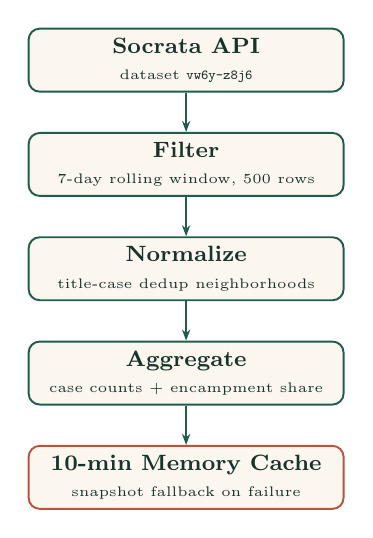
\begin{tikzpicture}[
        node distance=0.5cm,
        box/.style={
          rounded corners=4pt,
          draw=tenderlyForest,
          fill=tenderlyCream,
          text=tenderlyInk,
          minimum height=0.8cm,
          minimum width=4cm,
          align=center,
          font=\footnotesize,
          line width=0.7pt,
        },
        arr/.style={-{Stealth[length=4pt]}, tenderlyForest, line width=0.7pt},
      ]
        \node[box] (soc) {\textbf{Socrata API}\\{\tiny dataset \texttt{vw6y-z8j6}}};
        \node[box, below=of soc] (filter) {\textbf{Filter}\\{\tiny 7-day rolling window, 500 rows}};
        \node[box, below=of filter] (norm) {\textbf{Normalize}\\{\tiny title-case dedup neighborhoods}};
        \node[box, below=of norm] (agg) {\textbf{Aggregate}\\{\tiny case counts + encampment share}};
        \node[box, below=of agg, draw=tenderlyTerra] (cache) {\textbf{10-min Memory Cache}\\{\tiny snapshot fallback on failure}};

        \draw[arr] (soc) -- (filter);
        \draw[arr] (filter) -- (norm);
        \draw[arr] (norm) -- (agg);
        \draw[arr] (agg) -- (cache);
      \end{tikzpicture}
      \end{center}
    \end{column}
    \begin{column}{0.42\textwidth}
      \begin{block}{Data Rules}
        \begin{itemize}
          \item Freshness label with \texttt{updated\_at} timestamp
          \item Stale data labelled honestly, never faked as live
          \item Counts as directional context, not crisis claims
          \item Top 8 neighborhoods by case volume
          \item Top 3 categories per neighborhood
        \end{itemize}
      \end{block}
      \vspace{0.3cm}
      \begin{alertblock}{Fallback Guarantee}
        {\small If Socrata is unreachable, \texttt{needs\_snapshot.json} is served with the same contract shape --- the matching engine and UI never break.}
      \end{alertblock}
    \end{column}
  \end{columns}
\end{frame}

% ---------- database schema ----------
\begin{frame}{Data Model}
  \begin{center}
  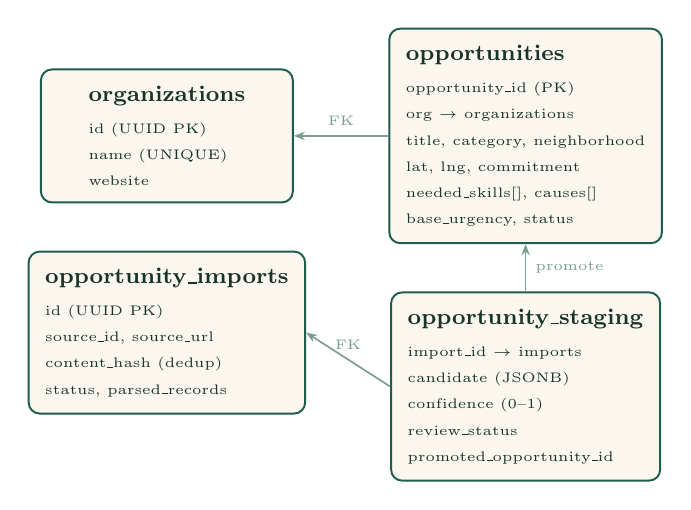
\begin{tikzpicture}[
    node distance=0.4cm and 1cm,
    tbl/.style={
      rounded corners=4pt,
      draw=tenderlyForest,
      fill=tenderlyCream,
      text=tenderlyInk,
      minimum width=3.2cm,
      align=left,
      font=\footnotesize,
      line width=0.7pt,
      inner sep=6pt,
    },
    arr/.style={-{Stealth[length=4pt]}, tenderlyForest!60, line width=0.6pt},
  ]
    \node[tbl] (org) {
      \textbf{organizations}\\[2pt]
      {\tiny id (UUID PK)}\\
      {\tiny name (UNIQUE)}\\
      {\tiny website}
    };

    \node[tbl, right=1.2cm of org] (opp) {
      \textbf{opportunities}\\[2pt]
      {\tiny opportunity\_id (PK)}\\
      {\tiny org $\rightarrow$ organizations}\\
      {\tiny title, category, neighborhood}\\
      {\tiny lat, lng, commitment}\\
      {\tiny needed\_skills[], causes[]}\\
      {\tiny base\_urgency, status}
    };

    \node[tbl, below=0.6cm of org] (imp) {
      \textbf{opportunity\_imports}\\[2pt]
      {\tiny id (UUID PK)}\\
      {\tiny source\_id, source\_url}\\
      {\tiny content\_hash (dedup)}\\
      {\tiny status, parsed\_records}
    };

    \node[tbl, below=0.6cm of opp] (stg) {
      \textbf{opportunity\_staging}\\[2pt]
      {\tiny import\_id $\rightarrow$ imports}\\
      {\tiny candidate (JSONB)}\\
      {\tiny confidence (0--1)}\\
      {\tiny review\_status}\\
      {\tiny promoted\_opportunity\_id}
    };

    \draw[arr] (opp.west) -- node[above, font=\tiny, text=tenderlyForest!60] {FK} (org.east);
    \draw[arr] (stg.west) -- node[above, font=\tiny, text=tenderlyForest!60] {FK} (imp.east);
    \draw[arr] (stg.north) -- node[right, font=\tiny, text=tenderlyForest!60] {promote} (opp.south);
  \end{tikzpicture}
  \end{center}

  \vspace{0.2cm}
  \centering
  {\small\color{tenderlyForest} Every recommendation traces back to an approved source and a specific parser run.}
\end{frame}

% ---------- closing ----------
\begin{frame}[plain]
  \begin{center}
    \vspace{2cm}
    {\Huge\bfseries\color{tenderlyInk} Tenderly}\\[0.6cm]
    {\large\color{tenderlyForest} When someone has the willingness to help,}\\[0.1cm]
    {\large\color{tenderlyForest} Tenderly turns uncertainty into a clear next step.}\\[1.5cm]
    {\normalsize\color{tenderlyTerra} Deployed on DigitalOcean App Platform}\\[0.2cm]
    {\small Powered by DigitalOcean AI Platform $\cdot$ Live SF 311 Open Data $\cdot$ PostgreSQL}
  \end{center}
\end{frame}

\end{document}
